\documentclass[a4paper,10pt]{article}
\usepackage{graphicx}
\usepackage{float}

% Title Page
\title{Assignment 1: Vacuum-Cleaning Agents}
\author{Francis Vo}


\begin{document}
\maketitle
% \{abstract}
Our goal was to study to preformance of different types of agents; Memory-less Deterministic Reflex Agent, Random Reflex Agent and Memory-Based Deteministic Reflex Agent.
We will measure the performance based on number of cleaned cells vs the number of actions taken.
The environment is a n X m empty rectangular room with p\% chance of containing dirt.
The agents have 5 actions; go forward, turn right by 90 degrees, turn left by 90 degrees, suck up dirt, and turn off.
The agents also have 3 sensor to interact with the room; a wall sensor, a dirt sensor, and a home sensor.
The memory-less Deterministic Reflex Agent

\section{Introduction}
AI background
Generic vacuum problem
Environment, partially observable, deterministic, single agent, sequential, discrete, known.
Agents-overview. Memory restrictions




\section{Problem Formulation}
Environment specifics

\section{Agents}
Describe the idea behind the design of each of your agents. Use diagrams and english as appropriate.
\subsection{Memory-less Deterministic Reflex Agent}
\subsubsection{Design}
\begin{figure}[H]
	\begin{center}
		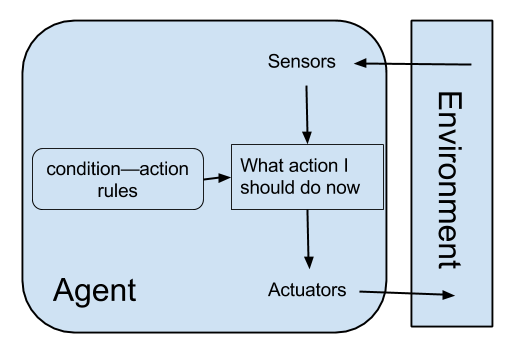
\includegraphics[width=0.6\textwidth]{MemorylessReflex.png}
	\end{center}
	% \caption{}
\end{figure}

The design for the memory-less deterministic reflex agent first uses its sensors to learn about its current location. Using that information, it follows condition-action rules to decide what to do next. The condition-action rules were designed to make the agent follow the wall around the room.

\subsubsection{If-then Rules}
\begin{verbatim}
if dirt then suck
else if wall then turn-right
else forward
\end{verbatim}

\subsubsection{Discussion}
What is the best possible performance achievable by any memory-less reflex agent in this domain? What prevents a memory-less reflex agent from doing very well in this task?

Since the agent follows the wall around the room, it will always run over 36 cells. 
So this means that it can only clean a maximum of 36 cells. 
It takes 37 forward actions to travel the room, not including 3 turn actions, then takes one action to turn off. 
This agent will always take 41 movement actions and a number of suck actions for the number of cells that were dirty on the side of the room. 
Therefore we can conclude the performance is:

\[\frac{\mbox{number of cleaned cells}}{\mbox{41 movement actions} + \mbox{number of cleaned cells}}\] 




\subsection{Random Reflex Agent}
How well does the random agent perform? Do you think that this is the best possible performance achievable by any random agent? Why or why not? Give a table showing the number of actions it took to clean 90\% of the room for each trial. What is the average of these numbers for the best 45 trials? What are the costs and benefits of randomness in agent design?
\subsubsection{Design}
\begin{figure}[H]
	\begin{center}
		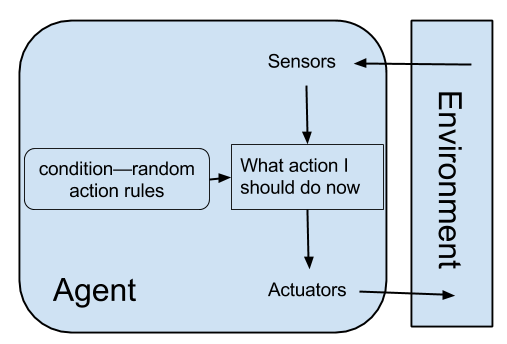
\includegraphics[width=0.6\textwidth]{RandomReflex.png}
	\end{center}
	% \caption{}
\end{figure}
\subsubsection{If-then Rules}
\begin{verbatim}
if dirt then suck
else if wall then turn-right 0.5 turn-left 0.5
else forward 0.5 turn-right 0.25 turn-left 0.25
\end{verbatim}


\subsection{Memory-Based Deterministic Reflex Agent}
How does the memory-based deterministic agent perform compared to the random agent? Was it able to completely clean the room? Was it able to shut itself off after it is done? If it did, how many actions did it take to do this? Can the agent be improved any further with more memory than you used? Why or why not?
\subsubsection{Design}
\begin{figure}[H]
	\begin{center}
		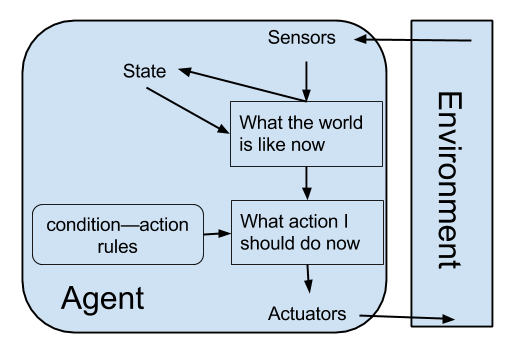
\includegraphics[width=0.6\textwidth]{MemoryReflex.png}
	\end{center}
	% \caption{}
\end{figure}

The memory-based deterministic reflex agent is similar to memory-less deterministic reflex agent, but it has more information about the world and its location with its 3-bit memory. 
This 3-bit memory allows the agent to know which direction its facing and if it took a turn recently.
In state 0, the agent knows that it is heading up.
In state 1, the agent knows that it just hit the north wall, and it is now facing right.
In state 2, the agent knows that it just turned after hitting the north wall, and it is facing right.
In state 3, the agent knows that it is now facing down. 
In state 4, the agent knows that it just hit the south wall, and it is now facing right.
In state 5, the agent knows that it just turned after hitting the south wall, and it is facing right.
In state 6, the agent knows that it just hit the east wall, now facing down, and on its way home.
In state 7, the agent knows that it just hit the south wall, now facing left, and on its way home.


\subsubsection{If-then Rules}
\begin{verbatim}
if dirt then suck
else if state0 and wall then turn-right set-state1
else if state1 and wall then turn-right set-state6
else if state1 and not wall then forward set-state2
else if state2 then turn-right set-state 3
else if state3 and wall then turn-left set-state4
else if state4 and wall then turn-right set-state6
else if state4 and not wall then forward set-state5
else if state5 then turn-left state-state0
else if state6 and wall then turn-right set-state7
else if state7 and home then off
else forward
\end{verbatim}


\section{Results}
Plots, discuss plots.

Plot 1- \%final dirt vs \% starting dirt \\
\begin{figure}[H]
	\begin{center}
		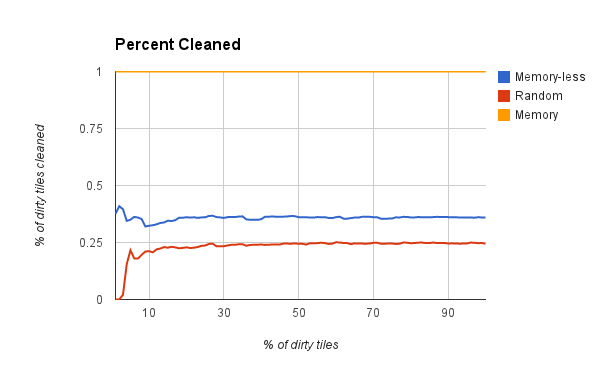
\includegraphics[width=0.9\textwidth]{image.png}
	\end{center}
	% \caption{}
\end{figure}
This graph measures the utility of each agent.
The utility is the usefulness of the agent to the user. 
The memory-based reflex agent always cleans 100\% of the dirt and therefore is very useful for the user.
The memoryless agent only cleans up to 36\% of the dirt because it only cleans the outer perimeter of the room.
The random agent cleaned a random 24\% of the dirt in the room. 

Plot 2- dirt per action vs \% starting dirt
\begin{figure}[H]
	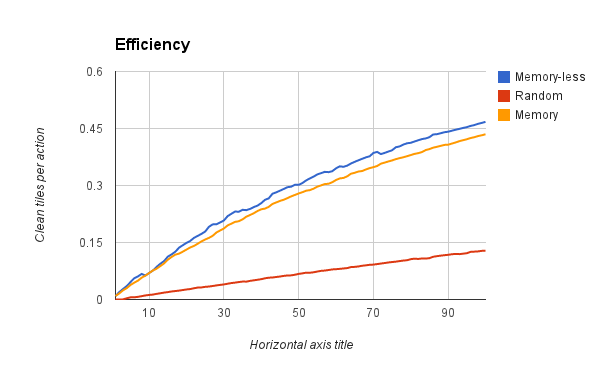
\includegraphics[width=0.9\textwidth]{image1.png}
\end{figure}



Plot 3- \# clean cells vs \# actions taken
\begin{figure}[H]
	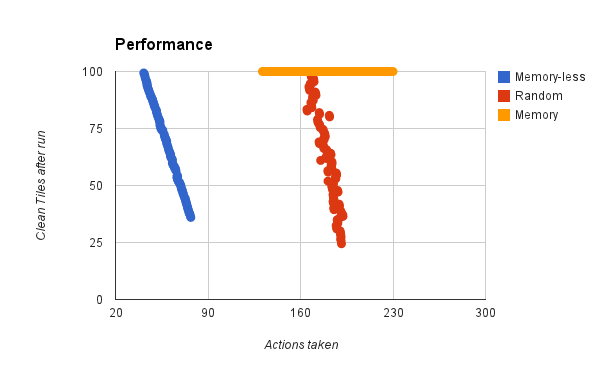
\includegraphics[width=0.9\textwidth]{image2.png}
\end{figure}

\section{Conclusion}
What did you learn from this experiment? Were you surprised by anything?
\end{document}
